\chapter{An\`{a}lisis i Especificaci\'{o}}
\label{cha:specification}
En aquest cap\'{i}tol s'analitzen les dades que gestiona Ichnaea i el comportament que es vol del sistema per cobrir les necessitats derivades de les execucions d'Ichnaea. D'aquest anàlisis es deriven els requeriments, les operatives que es necessiten i el model de dades.

\section{An\`{a}lisis de Requeriments}

\subsection{Requeriments funcionals}
\subsubsection{Administraci\'{o} d'usuaris}
La aplicaci\'{o} ha de estar protegida, auditada i autoritzada pels usuaris. Els usuaris autenticats han de tenir permisos i  pertànyer a grups amb rols autoritzats per fer certes accions dintre de l'aplicació web.\\ 

S'ha de dissenyar un sistema que permeti:
\begin{itemize}
\item Crear comptes d'usuari.
\item Atendre peticions de restaurar contrasenyes.
\item Enviament de correus electrònics de confirmacions de accions.
\item Canviar permisos a usuaris.
\end{itemize}

\subsubsection{Administraci\'{o} de variables de sistema}
La aplicaci\'{o} ha de gestionar les variables que Ichnaea utilitza per poder generar les entrades que necessita el \textit{software}. Aquestes variables han de tenir associades un o diversos conjunts de fitxers.\ref{cha:backgroud:univers:matrius:variables_seasons}).\\

S'ha de dissenyar un sistema que permeti:
\begin{itemize}
\item gestionar les variables que necessita Ichnaea.
\item gestionar els fitxers i el contingut dels fitxers que necessiten les variables.
\item gestionar les associacions entre els fitxers, els conjunts de fitxers i les variables .
\end{itemize} 

\subsubsection{Administraci\'{o} de matrius}
La aplicaci\'{o} ha de gestionar i configurar matrius de dades. Per la creaci\'{o} de matrius ha de poder llegir una fulla de c\`{a}lcul i crear un model de dades que representi una matriu a partir de les dades proporcionades. A mes, la aplicaci\'{o} ha de permetre la configuraci\'{o} de les matrius.(mirar \ref{cha:backgroud:univers:matrius})\\

S'ha de dissenyar un sistema permeti:
\begin{itemize}
\item gestionar matrius: crear, actualitzar, esborrar i configurar-les.
\item configurar les columnes d'una matriu com una variable i un conjunt de fitxers en cas de que tinguin m\'{e}s.
\item configurar l'origen d'una mostra de la matriu.
\item configurar la data d'una mostra de la matriu.
\item Configurar o actualitzar dades b\`{a}siques d'una matriu.
\end{itemize}

\subsubsection{Administraci\'{o} de entrenaments}
El sistema ha de gestionar i crear entrenaments i enviar-ho contra una cua d'execuci\'{o} d'Ichnaea. Per executar un entrenament s'ha de generar les dades d'entrada a partir de las matrius\ref{subsec:backgroundTrainings}.\\

S'ha de dissenyar un sistema que permeti:
\begin{itemize}
	\item gestionar els entrenaments: crear, configurar i esborrar.
	\item generar les dades necessaries per les execucions dels entrenaments.
	\item enviar les dades generades a la cua d'execucions d'entrenaments.
	\item llegir e interpretar l'estat del proc\'{e}s d'entrenament.
	\item guardar els resultats dels entrenaments.
	\item Gestionar les sortides de les execucions.
\end{itemize}

\subsubsection{Administraci\'{o} de matrius de predicci\'{o}}
El sistema ha de gestionar i crear noves matrius de prediccions. A m\'{e}s ha de generar les dades necessàries per executar prediccions i enviar-les a una cua d'execucions de prediccions.\\

S'ha de dissenyar un sistema que permeti:
\begin{itemize}
	\item gestionar les matrius de prediccions.
	\item enviar a les matrius de prediccions a la cua d'execucions.
	\item Llegir e interpretar el estat del proc\'{e}s d'execució.
	\item Llegir els resultats de les prediccions.
	\item Gestionar les sortides de les execucions.
\end{itemize}

\subsection{Requeriments no funcionals}
Els requeriments no funcionals son:
\begin{itemize}
\item Un sistema amb bon rendiment 
\item Un sistema que permeti l'escalabilitat en cas d'augment o disminució de recursos
\item Un sistema fàcil de mantenir per continuar la evolució i/o resolució de mal funcionaments.
\item Un sistema amb un disseny flexible per poder fer canvis.
\item Un sistema usable pels usuaris.
\item Un sistema robust als errors.
\end{itemize}

\section{Model de Casos d'us}
A continuació expliquem els actors que intervenen al sistema i els casos d'usos generats de l'anàlisi de requeriments.

\subsection{Actors}
La figura \ref{fig:actors} descriu els actors físics i lògics del sistema. A continuació els detallem.

\begin{itemize}
\item Usuari an\`{o}nim: usuari sense compte al sistema.
\item Usuari registrat: usuari amb compte al sistema.
\begin{itemize}
\item Propietari d'una matriu: usuari que ha creat una matriu.
\item Propietari d'un entrenament: usuari que ha creat un entrenament.
\item Propietari d'una predicci\'{o}: usuari que ha creat una matriu de predicci\'{o}.
\end{itemize}
\item Usuari administrador: usuari amb permisos administratius.
\item Cua: usuari l\'{o}gic(no \'{e}s una persona f\'{i}sica) dels sistema que gestiona les execucions.
\item Consumidor: usuari l\'{o}gic(no \'{e}s una persona f\'{i}sica) del sistema que gestiona les sortides de les execucions.
\item Sistema: sistema que rep les peticions i gestiona les sortides.
\end{itemize}

\begin{figure}[h]
  \centering
  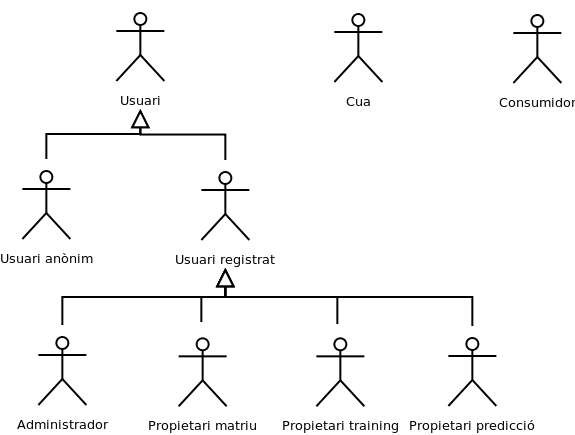
\includegraphics[scale=0.4]{img/specification/Actors.png}
  \caption{Diagrama d'actors dels sistema}
  \label{fig:actors}
\end{figure}

\subsection{Diagrama dels casos d'\'{u}s}
A la figura \ref{fig:usecases} es pot veure la el diagrama de casos d'\'{u}s. A la secció \ref{subsec:usescases} es detallen.
\begin{figure}[h]
  \centering
  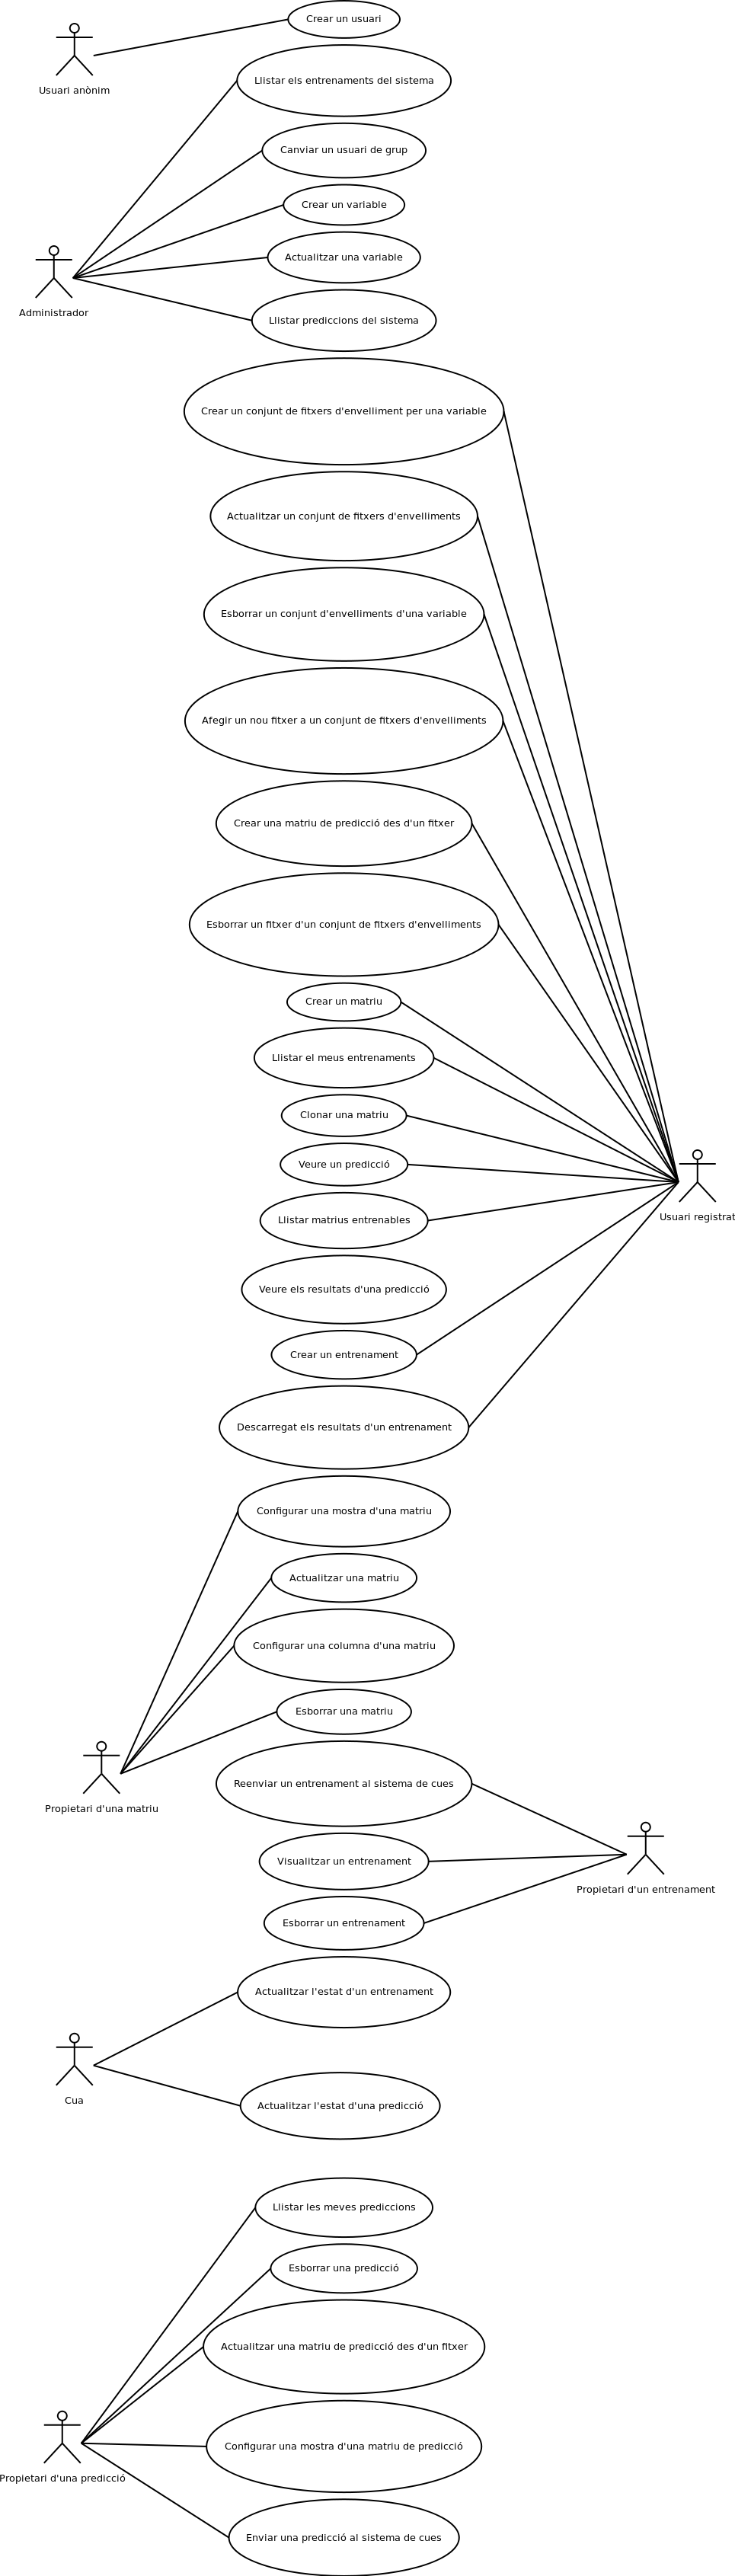
\includegraphics[scale=0.2]{img/specification/UsesCases.png}
  \caption{Diagrama de casos d'\'{u}s}
  \label{fig:usecases}
\end{figure}

\subsection{Especificaci\'{o} dels casos d'\'{u}s}
\label{subsec:usescases}
A continuació s'especifica el fluxe dels casos d'usos i el comportament del sistema en cadascun de ells. En la documentaci\'{o} s'utilitzar\`{a} la següent estructura per definir els casos d'\'{u}s:\\
\begin{usecase}
\addtitle{Identificador}{Nom cas d'us}
\addfield{Actors:}{Llista de actors}
\addscenario{Curs t\'{i}pic d'esdeveniments:}{
	\item Esdeveniment
	\item Esdeveniment
	\item ...
}
\addscenario{Cursos alternatius:}{
\item Esdeveniment Alternatiu
}
\end{usecase}


\begin{usecase}
\addtitle{Usuari001}{Crear un usuari}
\addfield{Actors:}{Anònim}
\addscenario{Curs t\'{i}pic d'esdeveniments:}{
	\item Usuari accedeix al formulari de registraci\'{o}. L'usuari introdueix un nom d'usuari, un correu electr\`{o}nic i una contrasenya per duplicat
	\item El sistema envia al usuari una confirmaci\'{o} via correu electr\'{o}nic amb un enllaç de confirmaci\'{o} i crea un compte no validada.
	\item L'usuari accedeix mitjançant l'enllaç de confirmaci\'{o}.
	\item El sistema comprova que \'{e}s un enllaç de confirmaci\'{o} v\`{a}lid d'aquest usuari i activa la compte. L'usuari ja est\'{a} autenticat com usuari bàsic del sistema.
}
\addscenario{Cursos alternatius:}{
\item[3] El sistema valida que no existeixi un usuari amb aquesta compte de correu i que el correu sigui v\`{a}lid. Sino \'{e}s correcte li informa a l'usuari al mateix formulari.
}
\end{usecase}

\begin{usecase}
\addtitle{Usuari002}{Canviar un usuari de grup}
\addfield{Actors:}{Administrador}
\addscenario{Curs t\'{i}pic d'esdeveniments:}{
	\item L'administrador llista tots els usuaris del sistema i selecciona un.
	\item El sistema mostra un formulari de edici\'{o} de permisos.
	\item L'administrador selecciona el nou permís i confirma l'acció.
	\item El sistema guarda els canvis i notifica a l'administrador.
}
\end{usecase}

\begin{usecase}
\addtitle{Variable001}{Crear una variable}
\addfield{Actors:}{Usuari administrador}
\addscenario{Curs t\'{i}pic d'esdeveniments:}{
	\item L'usuari accedeix a un formulari de creacio.
	\item El sistema mostra un formulari de creacio de variables.
	\item L'usuari dona un identificador i una descripci\'{o}.
	\item El sistema crea la variable amb la informació donada i confirma a l'usuari.
}
\addscenario{Cursos alternatius:}{
\item[4] El sistema valida que existeixi ja una variable amb aquest identificador i li notifica a l'usuari.
}
\end{usecase}

\begin{usecase}
\addtitle{Variable002}{Actualitzar una variable}
\addfield{Actors:}{Usuari administrador}
\addscenario{Curs t\'{i}pic d'esdeveniments:}{
    \item L'admininistrador seleccion un variable d'un llistat de variables.
    \item El sistema mostra un formulari d'edici\'{o} on pot veure els conjunts dels fitxers i pot actualitzar la descripci\'{o}.
    \item L'usuari modifica la descripci\'{o} i salva els canvis.
    \item El sistema guarda les modificacions.
}
\end{usecase}

\phantomsection
\label{variable003}
\begin{usecase}
\addtitle{Variable003}{Crear un conjunt de fitxers d'envelliment per una variable}
\addfield{Actors:}{Usuari registrat}
\addscenario{Curs t\'{i}pic d'esdeveniments:}{
	\item L'usuari selecciona una variable d'un llistat de variables.
	\item El sistema mostra un formulari d'edici\'{o} de la variable amb un enllaç a un formulari de creaci\'{o} de conjunt de fitxers.
	\item L'usuari accedeix a un formulari de creaci\'{o} d'un conjunt de fitxers.
	\item El sistema li mostra un formulari de creaci\'{o}.
	\item L'usuari pot donar un nom i seleccionar 0, 1 o 2 fitxers, on cada fitxer pot ser configurat com:
	\begin{itemize}
		\item a únic per tot l'any
		\item com estiu
		\item com hivern
		\item com tardor
		\item com estiu
	\end{itemize}	
	\item L'usuari salva els canvis.
	\item El sistema guarda els canvis i notifica a l'usuari.
}
\end{usecase}

\begin{usecase}
\addtitle{Variable004}{Actualitzar un conjunt de fitxers d'envelliments}
\addfield{Actors:}{Usuari registrat}
\addscenario{Curs t\'{i}pic d'esdeveniments:}{
    \item L'usuari selecciona una variable d'un llistat de variables.
    \item El sistema li mostra un llistat dels conjunts de fitxers de la variable.
    \item L'usuari selecciona un conjunt de fitxers.
    \item El sistema li mostra un formulari d'edició del conjunt de fitxers on es pot:
    \begin{itemize}
    \item Canviar el nom del conjunt de fitxers
    \item Esborrar un fitxer
    \item Afegir m\'{e}s fitxer i configurar-los com estiu, hivern, tardor, primavera o com tot l'any.
    \end{itemize}
    \item L'usuari salva els canvis.
    \item El sistema guarda els canvis i notifica a l'usuari. 
}
\end{usecase}

\begin{usecase}
\addtitle{Variable005}{Esborrar un conjunt d'envelliments d'una variable}
\addfield{Actors:}{Usuari registrat}
\addscenario{Curs t\'{i}pic d'esdeveniments:}{
    \item L'usuari selecciona una variable.
    \item El sistema mostra un llistat de conjunts de fitxers per esborrar.
    \item L'usuari selecciona del llistat un conjunt de fitxers per esborrar.
    \item El sistema li mostra un vista de confirmaci\'{o} de la acci\'{o}.
    \item L'usuari confirma la acci\'{o}.
    \item El sistema esborra tots els fitxers que no estiguin compartits i el conjunt.
}
\addscenario{Cursos alternatius:}{
\item[4] L'usuari cancel·la la acci\'{o}.
}
\addscenario{Cursos alternatius:}{
\item[6] El sistema avisa l'usuari que no pot esborrar el conjunt de fitxers ja que esta en us en una configuració de matrius.
}
\end{usecase}

\begin{usecase}
\addtitle{Variable006}{Afegir un nou fitxer a un conjunt de fitxers d'envelliments}
\addfield{Actors:}{Usuari registrat}
\addscenario{Curs t\'{i}pic d'esdeveniments:}{
    \item L'usuari selecciona una variable d'un llistat de variables.
    \item El sistema mostra un llistat de conjunts de fitxers de la variable.
    \item L'usuari seleccion un conjunt de fitxers.
    \item El sistema mostra un formulari de edici\'{o} del conjunt de fitxers.
    \item L'usuari pot seleccionar 0, 1 o 2 fitxers, on cada fitxer pot ser configurat com:
	\begin{itemize}
		\item a únic per tot l'any
		\item com estiu
		\item com hivern
		\item com tardor
		\item com estiu
	\end{itemize}
	\item L'usuari salva els canvis.
	\item El sistema guarda els canvis.
}
\end{usecase}

\begin{usecase}
\addtitle{Variable007}{Esborrar un fitxer d'un conjunt de fitxers d'envelliments}
\addfield{Actors:}{Usuari registrat}
\addscenario{Curs t\'{i}pic d'esdeveniments:}{
    \item L'usuari selecciona una variable d'un llistat de variables.
    \item El sistema mostra un llistat de conjunts de fitxers de la variable.
    \item L'usuari seleccion un conjunt de fitxers.
    \item El sistema mostra un llistat del fitxers.
	\item L'usuari selecciona un fitxer per esborrar.
	\item El sistema li demana confirmaci\'{o}.
	\item L'usuari confirma l'acci\'{o}
	\item El sistema esborra el fitxer.
}
\addscenario{Cursos alternatius:}{
\item[6] L'usuari cancel·la la acci\'{o}.
}
\addscenario{Cursos alternatius:}{
\item[8] El sistema notifica a l'usuari que no pot esborrar un fitxer que esta compartit amb un altre conjunt de fitxers.
}
\end{usecase}

\phantomsection
\label{variable008}
\begin{usecase}
\addtitle{Variable008}{Afegir un nou fitxer a un conjunt de fitxers d'envelliments}
\addfield{Actors:}{Usuari registrat}
\addscenario{Curs t\'{i}pic d'esdeveniments:}{
    \item L'usuari selecciona una variable d'un llistat de variables.
    \item El sistema mostra un llistat de conjunts de fitxers de la variable.
    \item L'usuari seleccion un conjunt de fitxers.
    \item El sistema mostra un formulari de edici\'{o} del conjunt de fitxers.
    \item L'usuari pot seleccionar 1 fitxer del sistema existent, on pot ser configurat com:
	\begin{itemize}
		\item a únic per tot l'any
		\item com estiu
		\item com hivern
		\item com tardor
		\item com estiu
	\end{itemize}
	\item L'usuari salva els canvis.
	\item El sistema guarda els canvis.
}
\end{usecase}

\begin{usecase}
\addtitle{Variable010}{Eliminar la associació d'un fitxer d'un conjunt de fitxers d'envelliments}
\addfield{Actors:}{Usuari registrat}
\addscenario{Curs t\'{i}pic d'esdeveniments:}{
    \item L'usuari selecciona una variable d'un llistat de variables.
    \item El sistema mostra un llistat de conjunts de fitxers de la variable.
    \item L'usuari seleccion un conjunt de fitxers.
    \item El sistema mostra un llistat del fitxers.
	\item L'usuari selecciona un fitxer per esborrar la associació.
	\item El sistema li demana confirmació.
	\item L'usuari confirma l'acci\'{o}
	\item El sistema esborra la associació però deixa el fitxer al sistema.
}
\addscenario{Cursos alternatius:}{
\item[6] L'usuari cancel·la la acci\'{o}.
}
\addscenario{Cursos alternatius:}{
\item[8] El sistema notifica a l'usuari que no pot esborrar un fitxer que esta compartit amb un altre conjunt de fitxers.
}
\end{usecase}

\phantonsection
\label{matriu001}
\begin{usecase}
\addtitle{Matriu001}{Crear una matriu des d'un fitxer}
\addfield{Actors:}{Usuari registrat}
\addscenario{Curs t\'{i}pic d'esdeveniments:}{
	\item L'usuari accedeix a un formulari de creació de matrius.
	\item El sistema mostra el formulari on pot donar nom a la matriu i seleccionar el fitxer en format CSV o Microsoft Excel. L'usuari accepta el formulari.
	\item El sistema crear la matriu on:
	\begin{itemize}
	\item La primera fila del fitxer s'associa com una variable Ichnaea. Si la variable es igual al identificador de la variable, automàticament s'assigna a aquesta columna a aquesta variable i a un conjunt de fitxers d'envelliments per defecte. Les dues ultimes columnes son optatives, on s'especifica l'origen i la data de la mostra.
	\item Cada fila del fitxer, despr\'{e}s de la primera fila:
	\begin{itemize}
		\item La primera columna \'{e}s l'identificador de la mostra. Si cont\'{e} un alias d'origen, autom\`{a}ticament s'assigna un origen
		\item Les columnes restants s'assignen com a valors de la mostra
		\item Les dos ultimes columnes seran l'origen o la data segons la primera fila del fitxer.
	\end{itemize}
	\item L'usuari visualitza la matriu.
	\end{itemize}
}
\end{usecase}

\begin{usecase}
\addtitle{Matriu002}{Actualitzar una matriu}
\addfield{Actors:}{Propietari de la matriu}
\addscenario{Curs t\'{i}pic d'esdeveniments:}{
	\item L'usuari selecciona una matriu per actualitzar.
	\item El sistema li mostra un formulari d'edici\'{o} de la matriu.
	\item L'usuari accedeix a un formulari de importacio.
	\item El sistema mostra el formulari d'edicio.
	\item L'usuari pot actualitzar el nom a la matriu i/o seleccionar el fitxer de tipus de fulla de c\`{a}lcul. L'usuari confirma els canvis
	\item El sistema esborra la matriu anterior i torna a crear la matriu on:
	\begin{itemize}
	\item La primera fila del fitxer s'associa com una variable Ichnaea. Si la variable es igual al identificador de la variable, automàticament s'assigna a aquesta columna a aquesta variable i a un conjunt de fitxers d'envelliments per defecte. Les dues ultimes columnes son optatives, on s'especifica l'origen i la data de la mostra.
	\item Cada fila del fitxer, despr\'{e}s de la primera fila:
	\begin{itemize}
		\item La primera columna \'{e}s l'identificador de la mostra. Si cont\'{e} un alias d'origen, autom\`{a}ticament s'assigna un origen
		\item Les columnes restants s'assignen com a valors de la mostra
		\item Les dos ultimes columnes seran l'origen o la data segons la primera fila del fitxer.
	\end{itemize}
	\end{itemize}
	\item L'usuari visualitza la matriu.
}
\end{usecase}

\begin{usecase}
\addtitle{Matriu003}{Clonar una matriu}
\addfield{Actors:}{Usuari registrat}
\addscenario{Curs t\'{i}pic d'esdeveniments:}{
	\item L'usuari selecciona una matriu per clonar.
	\item El sistema mostra un formulari amb un nom suggerit per la matriu.
	\item L'usuari pot canviar el nom i acceptar la clonaci\'{o}.
	\item El sistema clona la matriu i la seva configuraci\'{o} sense copiar entrenaments ni prediccions. El propietari de la matriu \'{e}s l'usuari que ha realitzat la clonaci\'{o}. 
	\item L'usuari veu la matriu clonada.
}
\end{usecase}

\begin{usecase}
\addtitle{Matriu004}{Esborrar una matriu}
\addfield{Actors:}{Propietari de la matriu}
\addscenario{Curs t\'{i}pic d'esdeveniments:}{
	\item L'usuari selecciona una matriu del sistema per esborrar.
	\item El sistema demana confirmaci\'{o} per esborrar la matriu.
	\item L'usuari confirma la acci\'{o}.
	\item El sistema clona la matriu i la seva configuraci\'{o} sense copiar entrenaments ni prediccions. El propietari de la matriu \'{e}s l'usuari que ha realitzat la clonaci\'{o}.
}
\addscenario{Cursos alternatius:}{
	\item[3] L'usuari cancel·la la acci\'{o}.
}
\end{usecase}

\phantonsection
\label{matriu005}
\begin{usecase}
\addtitle{Matriu005}{Configurar la columna d'una matriu}
\addfield{Actors:}{Usuari propietari de la matriu}
\addscenario{Curs t\'{i}pic d'esdeveniments:}{
	\item L'usuari selecciona una matriu
	\item El sistema mostra una vista per configurar les columnes de una matriu.
	\item L'usuari selecciona una columna i pot:
	\begin{itemize}
		\item donar un nom a la columna
		\item seleccionar una variable i una conjunt d'envelliments de la variable
	\end{itemize}
	\item L'usuari accepta la configuraci\'{o}
	\item El sistema salva la configuraci\'{o} de la columna
}
\end{usecase}

\begin{usecase}
\addtitle{Matriu006}{Configurar una mostra d'una matriu}
\addfield{Actors:}{Usuari propietari de una matriu}
\addscenario{Curs t\'{i}pic d'esdeveniments:}{
	\item L'usuari selecciona una matriu.
	\item El sistema mostra una vista per configurar les mostres de la matriu.
	\item L'usuari selecciona una mostra i pot:
	\begin{itemize}
	\item donar una data 
	\item donar una nom a la mostra
	\item donar un origen de la mostra
	\end{itemize}
	\item L'usuari accepta la configuraci\'{o}.
	\item El sistema guarda la configuraci\'{o} de la mostra.
}
\end{usecase}

\begin{usecase}
\addtitle{Matriu007}{Validar una matriu}
\addfield{Actors:}{Usuari propietari de una matriu}
\addscenario{Curs t\'{i}pic d'esdeveniments:}{
	\item L'usuari selecciona un matriu.
	\item El sistema mostra una vista per validar les dades.
	\item L'usuari accepta una validaci\'{o}.
	\item El sistema mostra al usuari si conte alguna dada buida com algun valor de mostres, un origen d'una mostra buit o una data de mostra buida.
}
\end{usecase}

\begin{usecase}
\addtitle{Training001}{Llistar els entrenaments del sistema}
\addfield{Actors:}{Usuari administrador}
\addscenario{Curs t\'{i}pic d'esdeveniments:}{
	\item L'usuari accedeix a la vista del llistat de entrenaments del sistema.
	\item El sistema llista els entrenaments amb les dades b\`{a}siques: 
	\begin{itemize}
	\item nom de la matriu entrenada
	\item estat del entrenament
	\item descripci\'{o} de l'entrenament
	\item creador de l'entrenament
	\item data de creaci\'{o} de l'entrenament.
	\end{itemize}
}
\end{usecase}

\begin{usecase}
\addtitle{Training002}{Llistar els meus entrenaments}
\addfield{Actors:}{Usuari registrat}
\addscenario{Curs t\'{i}pic d'esdeveniments:}{
	\item L'usuari accedeix a la vista del llistat de entrenaments que ha creat.
	\item El sistema llista els entrenaments que ha creat amb dades b\`{a}siques: 
	\begin{itemize}
	\item nom de la matriu entrenada
	\item estat de l'entrenament
	\item descripci\'{o} de l'entrenament
	\item data de creaci\'{o} de l'entrenament.
	\end{itemize}
}
\end{usecase}

\begin{usecase}
\addtitle{Training003}{Llistar matrius entrenables}
\addfield{Actors:}{Usuari registrat}
\addscenario{Curs t\'{i}pic d'esdeveniments:}{
	\item L'usuari accedeix a la vista del llistat de matrius entrenables.
	\item El sistema llista els entrenaments amb un estat finalitzat i sense errors amb dades b\`{a}siques: 
	\begin{itemize}
	\item nom de la matriu entrenada
	\item estat de l'entrenament
	\item creador
	\item descripci\'{o} de l'entrenament
	\item data de creaci\'{o}.
	\end{itemize}
}
\end{usecase}

\phantonsection
\label{training004}
\begin{usecase}
\addtitle{Training004}{Crear un entrenament}
\addfield{Actors:}{Usuari registrat}
\addscenario{Curs t\'{i}pic d'esdeveniments:}{
	\item L'usuari selecciona una matriu per entrenar.
	\item El sistema li mostra un formulari per crear entrenaments.
	\item L'usuari pot donar un nom, una descripci\'{o}, seleccionar un origen dels disponibles i quines columnes vol entrenar. Finalment confirma les dades.
	\item El sistema guarda l'entrenament i envia les dades al sistema de cues d'execucions de entrenaments. El sistema avalua si ha pogut enviar l'entrenament al sistema de cues en cas que el servei estigui caigut. 
	\item L'usuari veu les dades b\'{a}siques de l'entrenament.
}
\end{usecase}

\begin{usecase}
\addtitle{Training005}{Re-enviar un entrenament al sistema de cues}
\addfield{Actors:}{Usuari propietari d'un entrenament}
\addscenario{Curs t\'{i}pic d'esdeveniments:}{
    \item L'usuari selecciona un entrenament que ha tingut problemes de enviament.
    \item El sistema mostra una vista de visualitzaci\'{o} del entrenament.
    \item L'usuari pot consultar quin possible error ha passat i pot confirmar el re-enviament.
    \item El sistema actualitza les dades i re-envia les dades al sistema de cues.
}
\end{usecase}

\begin{usecase}
\addtitle{Training006}{Visualitzar un entrenament}
\addfield{Actors:}{Usuari registrat}
\addscenario{Curs t\'{i}pic d'esdeveniments:}{
    \item L'usuari selecciona d'un llistat un entrenament.
    \item El sistema mostra una vista de visualitzaci\'{o} de l'entrenament amb el nom, descripci\'{o}, data de creaci\'{o} i  errors o resultats segons el cas.
}
\end{usecase}

\begin{usecase}
\addtitle{Training007}{Esborrar un entrenament}
\addfield{Actors:}{Usuari superadministrador, usuari propietari d'un entrenament}
\addscenario{Curs t\'{i}pic d'esdeveniments:}{
	\item L'usuari selecciona un entrenament per esborrar.
	\item El sistema demana confirmaci\'{o} per esborrar l'entrenament.
	\item L'usuari confirma l'acci\'{o}
	\item El sistema esborra el entrenaments i totes les prediccions que s'han fet a partir d'aquest entrenament.
}
\addscenario{Cursos alternatius:}{
	\item[3] L'usuari cancel·la la acci\'{o}.
}

\end{usecase}

\begin{usecase}
\addtitle{Training008}{Descarregar els resultats d'un entrenament}
\addfield{Actors:}{Usuari registrat}
\addscenario{Curs t\'{i}pic d'esdeveniments:}{
    \item L'usuari selecciona un entrenament finalitzat.
    \item El sistema visualitza un enllaç amb la possibilitat de descarregar el fitxer resultats d'un entrenament.
    \item L'usuari accedeix a la descarrega.
    \item El sistema envia a l'usuari els resultats.
}
\end{usecase}

\begin{usecase}
\addtitle{Training009}{Actualitzar l'estat d'un entrenament}
\addfield{Actors:}{Cua}
\addscenario{Curs t\'{i}pic d'esdeveniments:}{
    \item La cua avisa al consumidor que ha finalitzat un entrenament i li envia les dades al consumidor.
    \item El consumidor rep les dades i li envia al sistema
    \item El sistema les guarda i actualitza l'estat del entrenament.
}
\end{usecase}

\begin{usecase}
\addtitle{Prediction001}{Llistar prediccions del sistema}
\addfield{Actors:}{Usuari administrador}
\addscenario{Curs t\'{i}pic d'esdeveniments:}{
	\item L'usuari accedeix a la vista del llistat de prediccions
	\item El sistema llista totes les prediccions amb dades b\`{a}siques:
	\begin{itemize}
	\item nom de la matriu
	\item nom de l'entrenament
	\item nom de la predicció
	\item data de creació
	\item estat de la execució.
	\end{itemize}
}
\end{usecase}

\begin{usecase}
\addtitle{Prediction002}{Llistar les meves prediccions}
\addfield{Actors:}{Usuari registrats}
\addscenario{Curs t\'{i}pic d'esdeveniments:}{
	\item L'usuari accedeix a la vista del llistat de prediccions creades per ell.
	\item EL sistema llista totes les prediccions creades per l'usuari amb dades b\`{a}siques.
		\begin{itemize}
	\item nom de la matriu
	\item nom de l'entrenament
	\item nom de la predicció
	\item data de creació
	\item estat de la execució.
	\end{itemize}
}
\end{usecase}

\begin{usecase}
\addtitle{Prediction003}{Esborrar una predicci\'{o}}
\addfield{Actors:}{Usuari registrats}
\addscenario{Curs t\'{i}pic d'esdeveniments:}{
	\item L'usuari selecciona una predicci\'{o} per esborrar.
	\item El sistema li demana confirmaci\'{o} per esborrar la predicci\'{o}.
	\item L'usuari confirma la acci\'{o}.
	\item El sistema esborra la predicci\'{o}.
}
\addscenario{Cursos alternatius:}{
	\item[3] L'usuari cancel·la la acci\'{o}.
}
\end{usecase}

\begin{usecase}
\addtitle{Prediction004}{Crear una matriu de predicci\'{o} des d'un fitxer}
\addfield{Actors:}{Usuari registrats}
\addscenario{Curs t\'{i}pic d'esdeveniments:}{
	\item L'usuari selecciona un entrenament per crear una predicci\'{o}.
	\item El sistema li mostra un formulari de creaci\'{o} de prediccions.
	\item L'usuari accedeix a un formulari on pot donar nom a la matriu de predicci\'{o} i seleccionar una fulla de c\`{a}lcul. L'usuari accepta el formulari.
	\item El sistema crea la matriu on:
	\begin{itemize}
	\item La primera fila del fitxer s'associa com una variable entrenada. Si la variable es igual al identificador de la variable entrenada, automàticament s'assigna a aquesta columna a aquesta columna de l'entrename i al un conjunt de fitxers d'envelliments que s'ha entrenat. Les dues ultimes columnes son optatives, on s'especifica l'origen i la data de la mostra.
	\item Cada fila del fitxer, despr\'{e}s de la primera fila:
	\begin{itemize}
		\item La primera columna \'{e}s l'identificador de la mostra. Si cont\'{e} un alias d'origen, autom\`{a}ticament s'assigna un origen
		\item Les columnes restants s'assignen com a valors de la mostra
		\item Les dos ultimes columnes seran l'origen o la data segons la primera fila del fitxer.
	\end{itemize}
	\end{itemize}
	\item El sistema mostra la matriu de predicció.
}
\end{usecase}

\begin{usecase}
\addtitle{Prediction005}{Actualitzar una matriu de predicci\'{o} des d'un fitxer}
\addfield{Actors:}{Usuari propietari de la predicci\'{o}}
\addscenario{Curs t\'{i}pic d'esdeveniments:}{
    \item L'usuari selecciona un entrenament.
    \item El sistema li mostra un formulari d'edici\'{o} de prediccions.
    \item L'usuari pot actualitzar el nom de la predicci\'{o} i seleccionar una fulla de c\'{a}lcul i guardar els canvis.
    \item El sistema esborra la matrius de predicci\'{o}, actualitza les dades i crea la matriu on:
	\begin{itemize}
	\item La primera fila del fitxer s'associa com una variable entrenada. Si la variable es igual al identificador de la variable entrenada, automàticament s'assigna a aquesta columna a aquesta columna de l'entrename i al un conjunt de fitxers d'envelliments que s'ha entrenat. Les dues ultimes columnes son optatives, on s'especifica l'origen i la data de la mostra.
	\item Cada fila del fitxer, despr\'{e}s de la primera fila:
	\begin{itemize}
		\item La primera columna \'{e}s l'identificador de la mostra. Si cont\'{e} un alias d'origen, autom\`{a}ticament s'assigna un origen
		\item Les columnes restants s'assignen com a valors de la mostra
		\item Les dos ultimes columnes seran l'origen o la data segons la primera fila del fitxer.
	\end{itemize}
	\end{itemize}

}
\end{usecase}

\subsubsection{Configurar una mostra d'una matriu de predicci\'{o}}
\begin{usecase}
\addtitle{Prediction 006}{Configurar una mostra d'una matriu de predicci\'{o}}
\addfield{Actors:}{Usuari propietari de la predicci\'{o}}
\addscenario{Curs t\'{i}pic d'esdeveniments:}{
	\item L'usuari selecciona una predicci\'{o} i una mostra.
	\item El sistema mostra una vista de edici\'{o} de la matriu.
	\item L'usuari pot donar un data, un nom i un origen a la mostra i guardar els canvis.
	\item El sistema guarda les dades.
}
\end{usecase}

\subsubsection{Enviar una predicci\'{o} al sistema de cues}
\begin{usecase}
\addtitle{Prediction007}{Enviar una predicci\'{o} al sistema de cues}
\addfield{Actors:}{Usuari propietari de la predicci\'{o}}
\addscenario{Curs t\'{i}pic d'esdeveniments:}{
    \item L'usuari selecciona una predicci\'{o}.
    \item El sistema li mostra un formulari per enviar la matriu de predicci\'{o} al sistema de cues.
    \item L'usuari confirma la acci\'{o}.
    \item El sistema prepara les dades per enviar i les envia al sistema de cues d'execucions de prediccions.
}
\end{usecase}

\subsubsection{Veure una predicci\'{o}}
\begin{usecase}
\addtitle{Prediction008}{Veure una predicci\'{o}}
\addfield{Actors:}{Usuari registrat}
\addscenario{Curs t\'{i}pic d'esdeveniments:}{
	\item L'usuari selecciona una predicci\'{o}.
	\item El sistema li mostra les dades b\`{a}siques de la predicci\'{o} i la matriu de predicci\'{o}.
}
\end{usecase}

\subsubsection{Veure els resultats d'una predicci\'{o}}
\begin{usecase}
\addtitle{Prediction009}{Veure els resultats d'una predicci\'{o}}
\addfield{Actors:}{Usuari registrat}
\addscenario{Curs t\'{i}pic d'esdeveniments:}{
	\item L'usuari selecciona els resultats d'una predicci\'{o}.
	\item El sistema li mostra les diferents sortides de la execuci\'{o}.
}
\end{usecase}

\phantonsection
\label{prediction010}
\subsubsection{Actualitzar l'estat d'una predicci\'{o}}
\begin{usecase}
\addtitle{Prediction010}{Actualitzar l'estat d'una predicci\'{o}}
\addfield{Actors:}{Cua, Consumidor}
\addscenario{Curs t\'{i}pic d'esdeveniments:}{
    \item La cua avisa al consumidor que ha finalitzat una predicci\'{o} i li envia les dades al consumidor
    \item El consumidor rep les dades i li envia al sistema
    \item El sistema les guarda i actualitza l'estat de la predicci\'{o}.
}
\end{usecase}

\subsubsection{Configurar una columna d'una matriu de predicció}
\begin{usecase}
\addtitle{Prediction011}{Actualitzar l'estat d'una predicci\'{o}}
\addfield{Actors:}{Propietari d'una predicció}
\addscenario{Curs t\'{i}pic d'esdeveniments:}{
   \item L'usuari selecciona una matriu de predicció.
   \item El sistema mostra una vista per configurar les columnes de una matriu de predicció.
	\item L'usuari selecciona una columna i pot:
	\begin{itemize}
		\item donar un nom a la columna
		\item seleccionar una variable amb el conjunt d'envelliments de la variable que s'ha entrenat.
	\end{itemize}
	\item L'usuari accepta la configuraci\'{o}
	\item El sistema salva la configuraci\'{o} de la columna i notifica a l'usuari.
}
\end{usecase}

\section{Model Conceptual}
A continuaci\'{o} es descriu el model conceptual resultant dels casos d'usos. Est\`{a} compost pel diagrama de classes i una explicació de cadascuna de les classes. 

\subsection{Diagrama de classes}
\label{subsec:diagramclasses}
La figura \ref{fig:datamodel} \'{e}s el diagrama UML\cite{uml} on est\`{a} implementat el modelatge de dades. Especifiquem el diagrama en angl\'{e}s per complir l'estandard UML.

\begin{sidewaysfigure}
  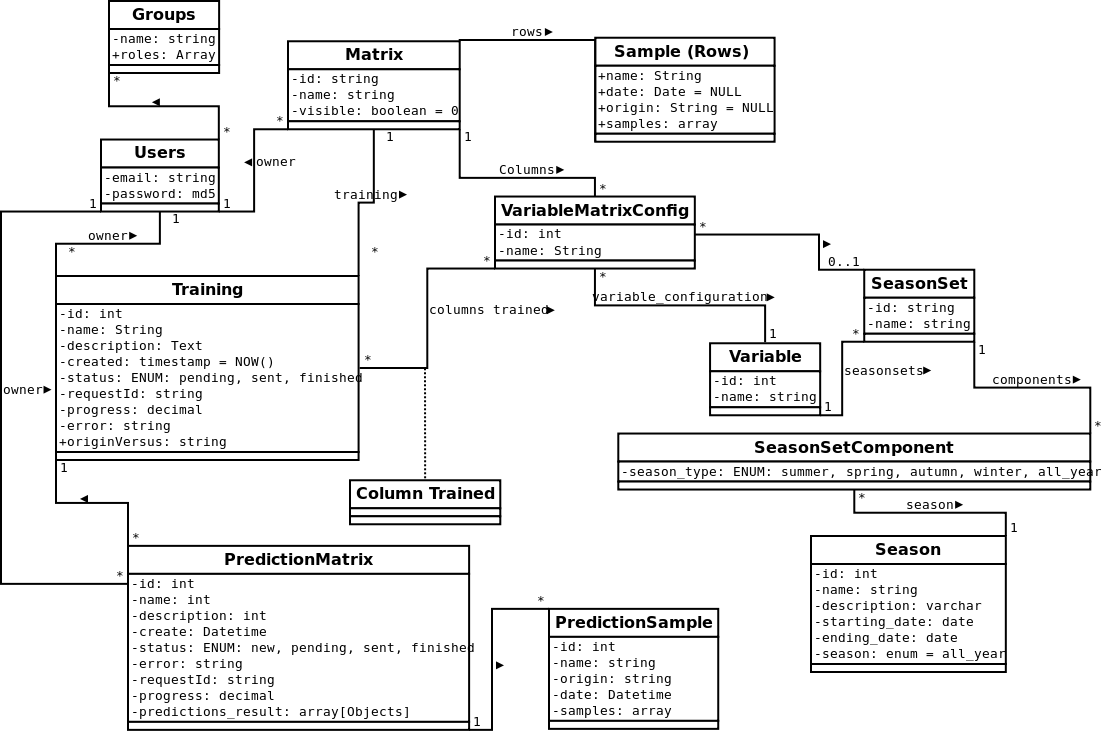
\includegraphics[scale=0.5]{img/specification/ModelClass.png}
  \caption{Model de dades}
  \label{fig:datamodel}
\end{sidewaysfigure}

Per la seva comprensió en la següent secció detallem el diagrama.


\subsection{Explicaci\'{o} de les classes}
A continuaci\'{o} es descriuran les classes del model de dades(figura \ref{fig:datamodel}), alguns atributs de les classes i les relacions entre elles.

\begin{itemize}
\item \textit{Users}: en aquesta classe es guarda la informaci\'{o} dels usuaris.

\item \textit{Groups}: en aquesta classe es guarda la informaci\'{o} dels grups. 

\item \textit{Season}: en aquesta classe es guarda la informaci\'{o} d'un fitxer d'envelliment.

\item \textit{SeasonSet}: en aquesta classe es guarda la informaci\'{o} d'un conjunt de fitxers.

\item \textit{SeasonSetComponent}: aquesta classe associa fitxers als conjunts de fitxers i quina es la seva configuració.

\item \textit{Matrix}: en aquesta classe es guarda la informaci\'{o} b\`{a}sica d'una matriu.

\item \textit{Sample}: en aquesta classe es guarda la informaci\'{o} de cadascuna de les files de la matriu a la que pertany mitjançant la associaci\'{o} \textit{rows}.

\item \textit{VariableMatrixConfig}: aquesta classe guarda la configuraci\'{o} d'una columna de la matriu i associa la columna amb una variable i amb un conjunt de fitxers d'aquesta variable.

\item \textit{Training}: en aquesta classe es guarda la informaci\'{o} d'un entrenament on:
\begin{itemize}
\item requestId: identificador del proc\'{e}s en la cua d'execuci\'{o}.
\item status: estat de la predicci\'{o}. Mirar l'apartat \ref{sec:status}.
\end{itemize}

\item \textit{Column Selected}: aquesta classe associa un entrenament amb quines columnes es volen entrenar.

\item \textit{PredictionMatrix}: en aquesta classe es guarda la informaci\'{o} d'una matriu de predicci\'{o} on:
\begin{itemize}
\item requestId: identificador del proc\'{e}s en la cua d'execuci\'{o}.
\item predictionResult: collecci\'{o} de resultats de la execuci\'{o} d'una predicci\'{o}.
\item status: estat de la predicci\'{o}. Mirar \ref{sec:status}.
\end{itemize}

\item \textit{PredictionSample}: en aquesta classe es guarda la informaci\'{o} de les mostres(files) d'una matriu de predicci\'{o}.

\item \textit{PredictionColumn}: en aquesta classe es guarda la informaci\'{o} de les columnes d'una matriu de predicci\'{o} i la associaci\'{o} entre les columnes entrenades. La propietat index cont\'{e} la posició que ocupa en la matriu.
\end{itemize}

\section{Model d'estats}
\label{sec:status}
La aplicaci\'{o} i el sistema de cues de execucions son dos components separats. Aix\'{o} ens obliga a definir estats per els entrenaments i per les prediccions.\\

El principal problema que existeix en la versi\'{o} actual de Ichnaea Software \'{e}s que no retorna estats parcials d'execucions: no ens retorna si ha començat la execució, quan temps queda o percentatge porta. A continuaci\'{o} s'explica quins estats s'han definit per els entrenaments i per les prediccions.

\subsection{Estats dels entrenaments}
\begin{figure}[H]
  \centering
  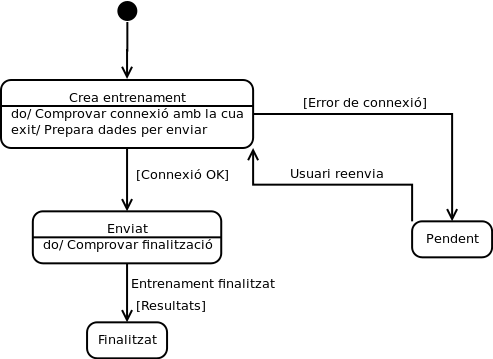
\includegraphics[scale=0.4]{img/specification/StatesTraining.png}
  \caption{Diagrama d'estats dels entrenaments}
  \label{fig:statestraining}
\end{figure}
Per crear un entrenament, primer es comprova que es pot establir connexi\'{o} amb la cua. Si no \'{e}s pot, l'entrenament queda marcat amb l'estat ''pendent''. En el cas que es pugui establir connexi\'{o}, s'envien les dades i es queda en aquest estat fins que li arribi algun esdeveniment de finalitzaci\'{o} amb els resultats o amb un error d'Ichnaea.\\

En el cas que estigui pendent, l'usuari podr\'{a} re-intentar enviar l'entrenament a la cua despr\'{e}s de comprovar l'error.

\subsection{Estats de les prediccions}
\begin{figure}[H]
  \centering
  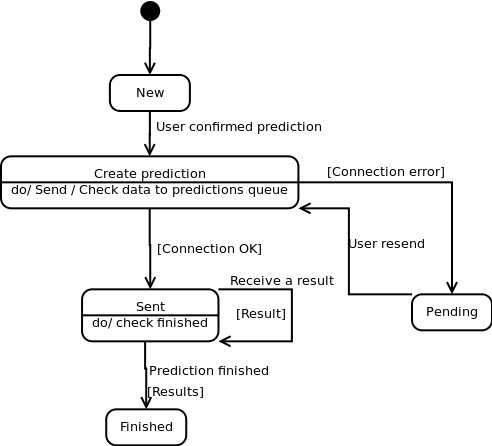
\includegraphics[scale=0.4]{img/specification/StatesPrediction.png}
  \caption{Diagrama d'estats dels entrenaments}
  \label{fig:statestraining}
\end{figure}
Per crear una predicci\'{o}, primer s'ha de configurar la matriu. Mentre l'usuari estigui configurant la matriu de predicci\'{o} estar\'{a} en un estat inicial(''nou''). Quan l'usuari confirmi l'enviament, primer es comprova que es pot establir connexi\'{o} amb la cua d'execucions de prediccions. Si no \'{e}s pot, l'entrenament queda marcat amb l'estat pendent. En el cas que es pugui establir connexi\'{o}, s'envien les dades. Es queda en aquest estat rebent múltiples respostes fins que li arribi algun esdeveniment de finalitzaci\'{o} amb els resultats o amb els errors.\\
En el cas que estigui pendent, l'usuari podr\'{a} re-intentar enviar la predicci\'{o} a la cua despr\'{e}s de comprovar l'error.

\section{Model del comportament}
En aquesta secci\'{o} veurem els diagrames de seqüència de les operacions m\'{e}s complexes dels casos d'us tenint en compte els estats definits.

\subsection*{Crear un conjunt de fitxers d'envelliments per una variable}
L'identificador d'aquest cas d'us \'{e}s \textbf{Variable003}(mirar la p\`{a}gina \pageref{variable003}).
\begin{figure}[H]
  \centering
  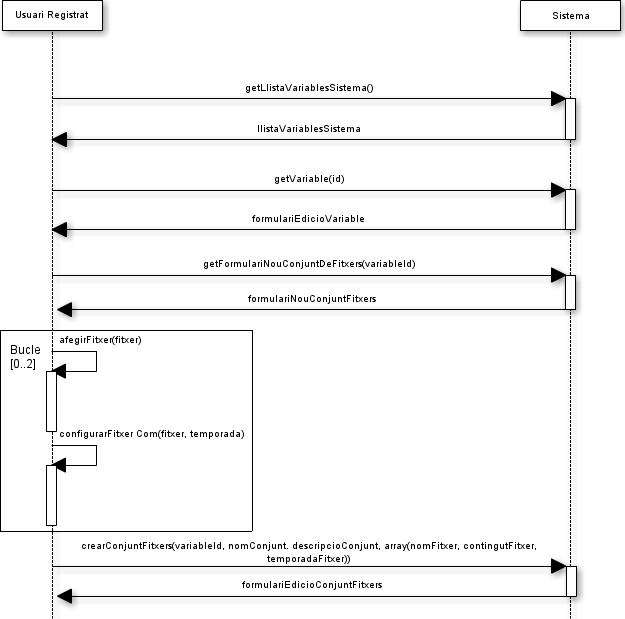
\includegraphics[scale=0.6]{img/specification/SequenceNewSeasonSe.png}
  \caption{Diagrama de seqüència \textit{Crear un conjunt de fitxers d'envelliments per una variable}}
  \label{fig:sequencenewseasonset}
\end{figure}

\subsection*{Afegir un nou fitxer a un conjunt de fitxers d'envelliments}
L'identificador d'aquest cas d'us \'{e}s \textbf{Variable008}(mirar la p\`{a}gina \pageref{variable008}).
\begin{figure}[H]
  \centering
  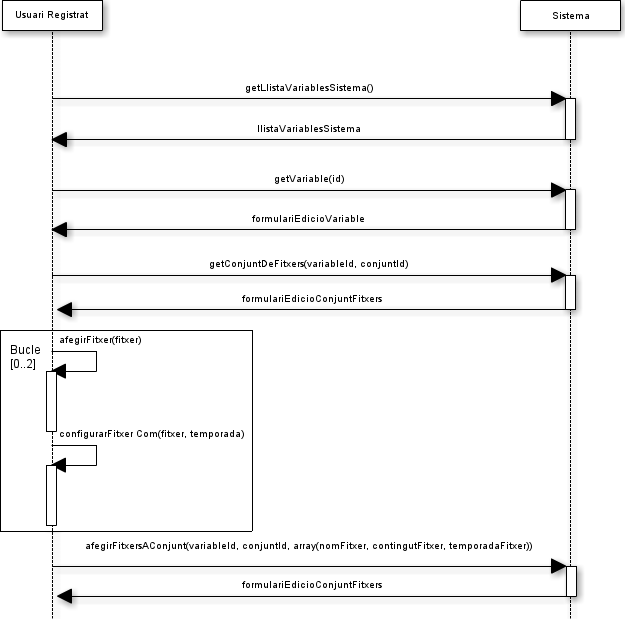
\includegraphics[scale=0.6]{img/specification/SequenceAddNewFilesToSeasonSet.png}
  \caption{Diagram de seqüència \textit{Afegir un nou fitxer a un conjunt de fitxers d'envelliments}}
  \label{fig:sequenceaddnewseason}
\end{figure}

\subsection*{Crear una matriu des d'un fitxer}
L'identificador d'aquest cas d'us \'{e}s \textbf{Matriu001}(mirar la p\`{a}gina \pageref{matriu001}).
\begin{figure}[H]
  \centering
  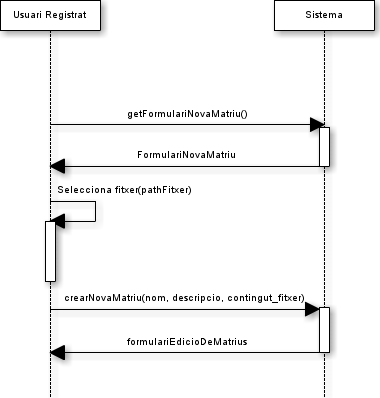
\includegraphics[scale=0.6]{img/specification/SequenceCreateMatrix.png}
  \caption{Diagram de seqüència \textit{Crear una matriu des d'un fitxer}}
  \label{fig:sequencenewmatrixfromfile}
\end{figure}

\subsection*{Crear un entrenament}
L'identificador d'aquest cas d'us \'{e}s \textbf{Training004}(mirar la p\`{a}gina \pageref{training004}).
\begin{figure}[H]
  \centering
  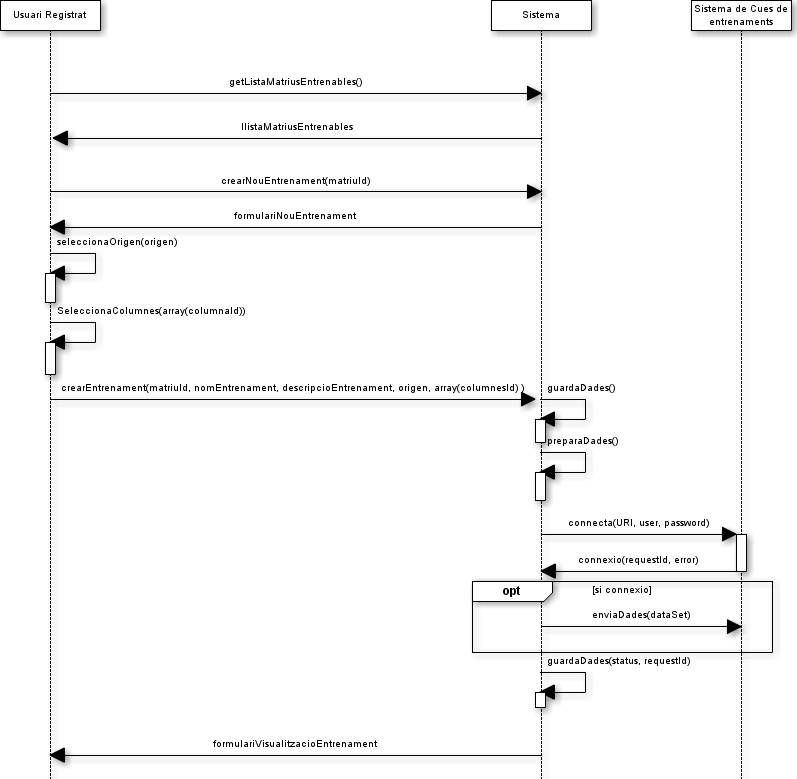
\includegraphics[scale=0.5]{img/specification/SequenceCreateTraining.png}
  \caption{Diagram de seqüència \textit{Crear un entrenament}}
  \label{fig:sequenceaddtraining}
\end{figure}

\subsection*{Configurar una columna d'una matriu}
L'identificador d'aquest cas d'us \'{e}s \textbf{Matriu005}(mirar la p\`{a}gina \pageref{matriu005}).
\begin{figure}[H]
  \centering
  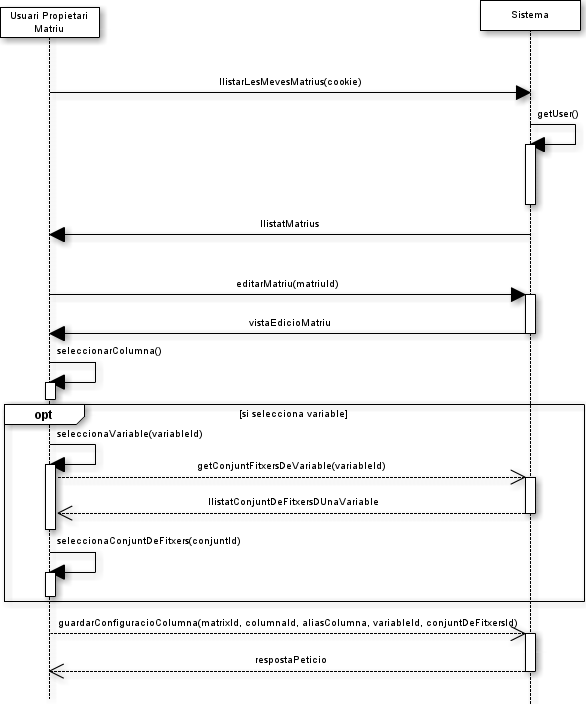
\includegraphics[scale=0.6]{img/specification/SequenceConfigureColumn.png}
  \caption{Diagrama de seqüencia \textit{Configurar una columna d'una matriu} }
  \label{fig:sequenceconfigurecolumn}
\end{figure}

\subsection*{Actualitzar l'estat d'una predicci\'{o}}
L'identificador d'aquest cas d'us \'{e}s \textbf{Prediction010}(mirar la p\`{a}gina \pageref{prediction010}).
\begin{figure}[H]
  \centering
  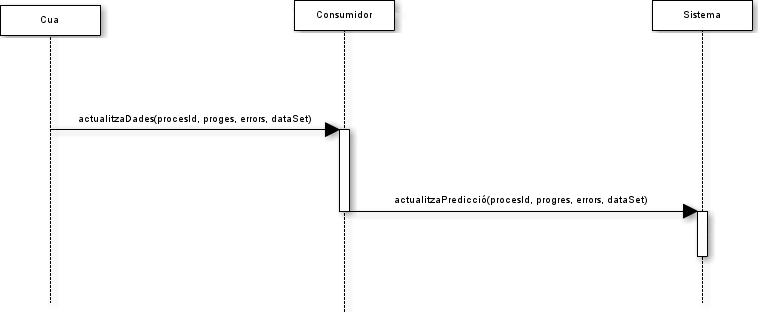
\includegraphics[scale=0.6]{img/specification/SequenceUpdatePrediccio.png}
  \caption{Diagrama de seqüencia \textit{Actualitzar l'estat d'una predicci\'{o}} }
  \label{fig:sequenceupdateprediccio}
\end{figure}
